






\section{Komposition von Abbildungen}

\textbf{Definition (Komposition):}\\
Seien $f:\mathbb{D}_f\longmapsto\mathbb{W}_f$ und $g:\mathbb{D}_g\longmapsto\mathbb{W}_g$ zwei Abbildungen, dann heißt die Abbildung:\\
\begin{align*}
	g\circ f: \mathbb{D}_f\longmapsto\mathbb{W}_g
\end{align*}
die Komposition von $f$ und $g$.\\
\begin{center}
	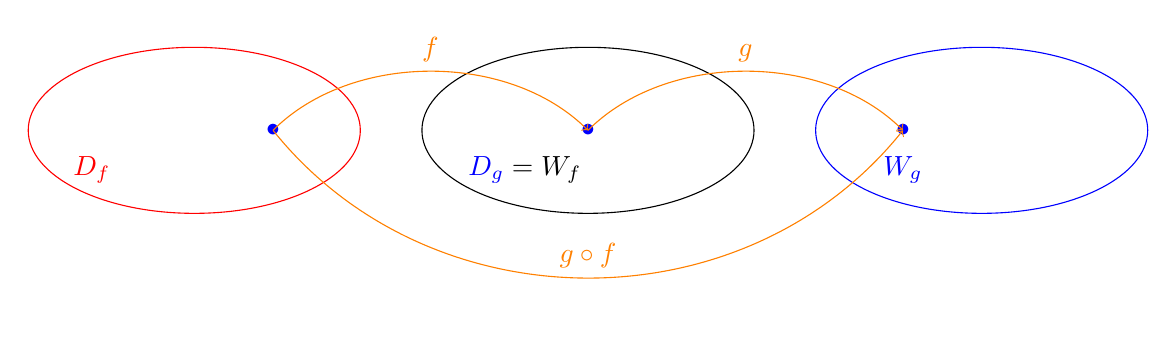
\begin{tikzpicture} 
		\draw[color=black] (5,0) ellipse (60pt and 30pt); 
		\draw[color=red] (0,0) ellipse (60pt and 30pt);
		\draw[color=blue] (10,0) ellipse (60pt and 30pt);
		%\draw[color=green] (5.5,0) ellipse (25pt and 15pt);
		
		\draw[color=black] (4.2,-.5) node { $\textcolor{blue}{\mathbb{D}_g}=\mathbb{W}_f$};
		\draw[color=red] (-1.3,-.5) node { $\mathbb{D}_f$};
		\draw[color=blue] (9,-0.5) node { $\mathbb{W}_g$};
		%\draw[color=green] (5.7,0) node { $\mathbb{V}$};
		\draw[color=blue,thick](1,0) node {$\bullet$};
		\draw[color=blue,thick](5,0) node {$\bullet$};
		\draw[color=blue,thick](9,0) node {$\bullet$};
		\draw[->,orange] (1, 0) .. controls(2, 1) and(4,1) .. node[above,sloped] {$f$}(5, 0);
		\draw[->,orange] (5, 0) .. controls(6, 1) and(8,1) .. node[above,sloped] {$g$}(9, 0);
		
		\draw[->,orange] (1, 0) .. controls(3, -2.5) and(7,-2.5) .. node[above,sloped] {$g\circ f$}(9, 0);
	\end{tikzpicture}
	
\end{center}
Ablauf der Komposition $g\circ f$:\\
Zuerst wird die Abildung $\mathbb{D}_f\longmapsto\mathbb{W}_f$ durchgeführt. Die Werte von $\mathbb{W}_f$ werden dann für die Abbildung $\mathbb{D}_g\longmapsto\mathbb{W}_g$ verwendet. Deshalb müssen mindestens die Werte von $\mathbb{W}_f$ in der Menge $\mathbb{D}_g$ enthalten sein. Sonst wäre ja eine Abbildung von $\mathbb{D}_g\longmapsto \mathbb{W}_g$ nicht möglich. Daraus folgt Wertebereich und Definitionsbereich beachten und es muss gelten:\\
\begin{align*}
	\mathbb{W}_f\subseteq \mathbb{D}_g
\end{align*}
Beispiel:\\
Sei:

\textbullet $\;\;f:]0,1]\longmapsto[1,\infty[$ mit $x\longmapsto \frac{1}{x}$\\

\textbullet $\;\,g:[0,\infty[ \longmapsto [0,\infty[$ mit $x\longmapsto\sqrt{x}$\vspace*{2mm}\\
Bilde:\\
(i) $\;g\circ f$\\
(ii) $f\circ g$\vspace*{2mm}\\
zu (i):\\
\begin{quote}
	Bilde $g\circ f$ mit:\\
	$f:\;\;]0,1] \longmapsto [1,\infty[$ mit $x\longmapsto\frac{1}{x}$\\
	$\mathbb{D}_f=]0,1]$\\
	$\mathbb{W}_f=[1,\infty[$\vspace*{2mm}\\
	$g:[0,\infty[ \longmapsto [0,\infty[$ mit $x\longmapsto\sqrt{x}$\\
	$\mathbb{D}_g=[0,\infty[$\\
	$\mathbb{W}_g=[0,\infty[$\vspace*{2mm}\\
	$g\circ f=\mathbb{D}_f\longmapsto\mathbb{W}_g$ dabei muß gelten: $\mathbb{W}_f\subseteq\mathbb{D}_g$\\
	$\mathbb{W}_f=[1,\infty[\;\subseteq\mathbb{D}_g=[0,\infty[$\vspace*{2mm}\\
	$g\circ f:\;\;]0,1]\longmapsto [0,\infty[$ mit $x\overset{f}{\longmapsto} \frac{1}{x}\overset{g}{\longmapsto}\sqrt{\scriptscriptstyle\frac{1}{x}}$\\
	$g\circ f:\;\;]0,1]\longmapsto [0,\infty[$ mit $x\overset{f\circ g}{\longmapsto} \sqrt{\scriptscriptstyle\frac{1}{x}}$\\ 
	
\end{quote}
\newpage
\noindent
zu (ii):\\
\begin{quote}
	Bilde: $f\circ g$ mit:\\
	$g:[0,\infty[ \longmapsto [0,\infty[$ mit $x\longmapsto\sqrt{x}$\\
	$\mathbb{D}_g=[0,\infty[$\\
	$\mathbb{W}_g=[0,\infty[$\vspace*{2mm}\\
	$f:\;\;]0,1] \longmapsto [1,\infty[$ mit $x\longmapsto\frac{1}{x}$\\
	$\mathbb{D}_f=]0,1]$\\
	$\mathbb{W}_f=[1,\infty[$\vspace*{2mm}\\
	$f\circ g=\mathbb{D}_g\longmapsto\mathbb{W}_f$ dabei muß gelten: $\mathbb{W}_g\subseteq\mathbb{D}_f$\\
	$\mathbb{W}_g=[0,\infty[\;\nsubseteq\mathbb{D}_f=]0,1]$\\
	$f\circ g:\;\;[0,\infty[ \longmapsto [1,\infty[$ ist nicht durchführbar!\\
	$f\circ g:\;\;[0,\infty[\longmapsto [1,\infty[$ mit $x\overset{g}{\longmapsto}\sqrt{x}\overset{f}{\longmapsto} \frac{1}{\sqrt{x}}$ nicht zulässig, weil die Null nicht eingesetzt werden darf. ($x\overset{f\circ g}{\longmapsto}=\frac{1}{\sqrt{x}}$)\\
\end{quote}
\subsection{Aufgabe zur Komposition von Abbildungen}

%\textbf{Definition (Komposition):}\\
\begin{tabular}[t]{lll}% l=linksbündig r=rechtsbündig
	Betrachte:&\\
	& $f:\mathbb{R}\longmapsto\mathbb{R}$ mit $x\longmapsto 1+x^4$ mit \\
	& $h:\mathbb{R}\longmapsto\mathbb{R}$ mit $x\longmapsto 1+x^3$ \\	
\end{tabular} \\
\begin{tabular}[t]{ll}% l=linksbündig r=rechtsbündig
	(i) & Existiert Funktion $g$ mit $h=g\circ f$ \\
	(ii) & Existiert Funktion $g$ mit $h=f\circ g$ \\	
\end{tabular} \vspace*{2mm}\\
zu (i):\\
\begin{quote}
	Gesucht: $g$ mit $h=g\circ f$\\
	$f(x)=1+x^4$\\
	$h(x)=1+x^3$\\
	$h(x)=(g\circ f)(x)\Leftrightarrow 1+x^3=g(f(x))=g(1+x^4) $\\
	\begin{align*}
		g(x)=1+(\sqrt[4]{x-1})^3
	\end{align*}
	Wie kommt man darauf?\\
	$g(x)=?$\\
	$1+x^4$ wird ja in  $g(x)$ eingesetzt.\\
	$g(x)$ soll $1+x^3$ rauskommen.\\
	wenn $g(x)= x-1$ dann ist $g(x)=1+x^4-1=x^4$ , wenn man $1+x^4$ einsetzt.\\
	Ziehe ich jetzt noch die 4 Wurzel, dann ist $g(x)=\sqrt[4]{x-1}$.
	Setzt man $1+x^4$ hier ein dann ist $g(x)=x$.\\
	Potenziert man dann die $\sqrt[4]{x-1}$ mit 3, dann ist $g(x)=(\sqrt[4]{x-1})^3$\\
	setzt man $1+x^4$ in $g(x)=(\sqrt[4]{x-1})^3$ ein, dann ist $g(x)=x^3$.\\
	Jetzt fehlt noch die 1 und die addiert man dazu, dann ist $g(x)=1+(\sqrt[4]{x-1})^3$ die Lösung.\\
	Antwort: \\
	Ja es gibt eine Funktion $g(x)$ mit $g(x):[1,\infty[\longmapsto[1,\infty[$ mit $x\longmapsto 1+(\sqrt[4]{x-1})^3$ 
\end{quote}
zu (ii):\\
\begin{quote}
	Gesucht: $g$ mit $h=f\circ g$\\
	$f(x)=1+x^4$\\
	$h(x)=1+x^3$\\
	$h(x)=(f\circ g)(x)\Leftrightarrow 1+x^3=f(g(x))\Leftrightarrow 1+x^3=1+(g(x))^4$\\
	bei $(g(x))^4$ muß ja $x^3$ rauskommen, also wählt man für $g(x)=\sqrt[4]{x^3}=x^{\frac{3}{4}}$\\
	\begin{align*}
		g(x)=x^{\frac{3}{4}}
	\end{align*}
	Antwort: \\Ja es gibt eine Funktion $g(x)$ mit $g(x):[0,\infty[\longmapsto[0,\infty[$ mit $x\longmapsto x^{\frac{3}{4}}$
\end{quote}

